\section{Multi-class detection policy}
We present a system that deploys multiple detectors to localize all object instances in the image.
The detectors are considered black boxes to the system, but it can measure the statistics of their performance at training time.

Our evaluation approach is explained in more details in Section \ref{sec:evaluation}; here we briefly summarize:
\begin{itemize}
\item The performance of the system is evaluated in the multi-class setting, meaning that detected boxes of a given class are matched to ground truth boxes of all classes, with the corresponding additional capacity for false positives.
\item The underlying performance metric is Average Precision: the area under the Precision vs. Recall curve.
\item Running a detector takes time and generates a list of detections, which are added to all current detections and thus generate a new AP point.
\item The system receives a start time and deadline; we seek to maximize the area under the AP vs. Time curve between these times.
\end{itemize}

Because the system must deliver results on a time budget, the policy must dynamically decide which detector in its arsenal to deploy next.
A symbolic explanation of the policy operation is shown in Figure \ref{fig:pomdp}.
To leverage the signal present in inter-object context, the decision of which detector to run next should be based on the observed results of detector actions that have already been run.
Of course, the observed results of detector actions do not give full confidence to the presence of a class in the image, necessitating an intermediate step from detection statistics to class presence in our system.

First, we look at how to construct such a system with only one detector per class.
We explain the general partially-observable decision process that we face and our choices for the different modular components of it.
We evaluate different ways of obtaining probabilities of object presence, and of estimating the value of running actions.
Next, we generalize the system to be able to handle multiple detector types per class, and show results on this task.

\section{Policy with a single detector per class}
The structure of the problem may be further defined as follows.
There are $|A|$ actions $a_i$.
Although we relax this later, at first we assume that each action consists in running a detector, and so generates a (possibly empty) list of detections when taken.
The same action will always generate the same list of detections, so there is no reason to ever take the same action more than once.

\begin{figure}[htb!]
  \centering
    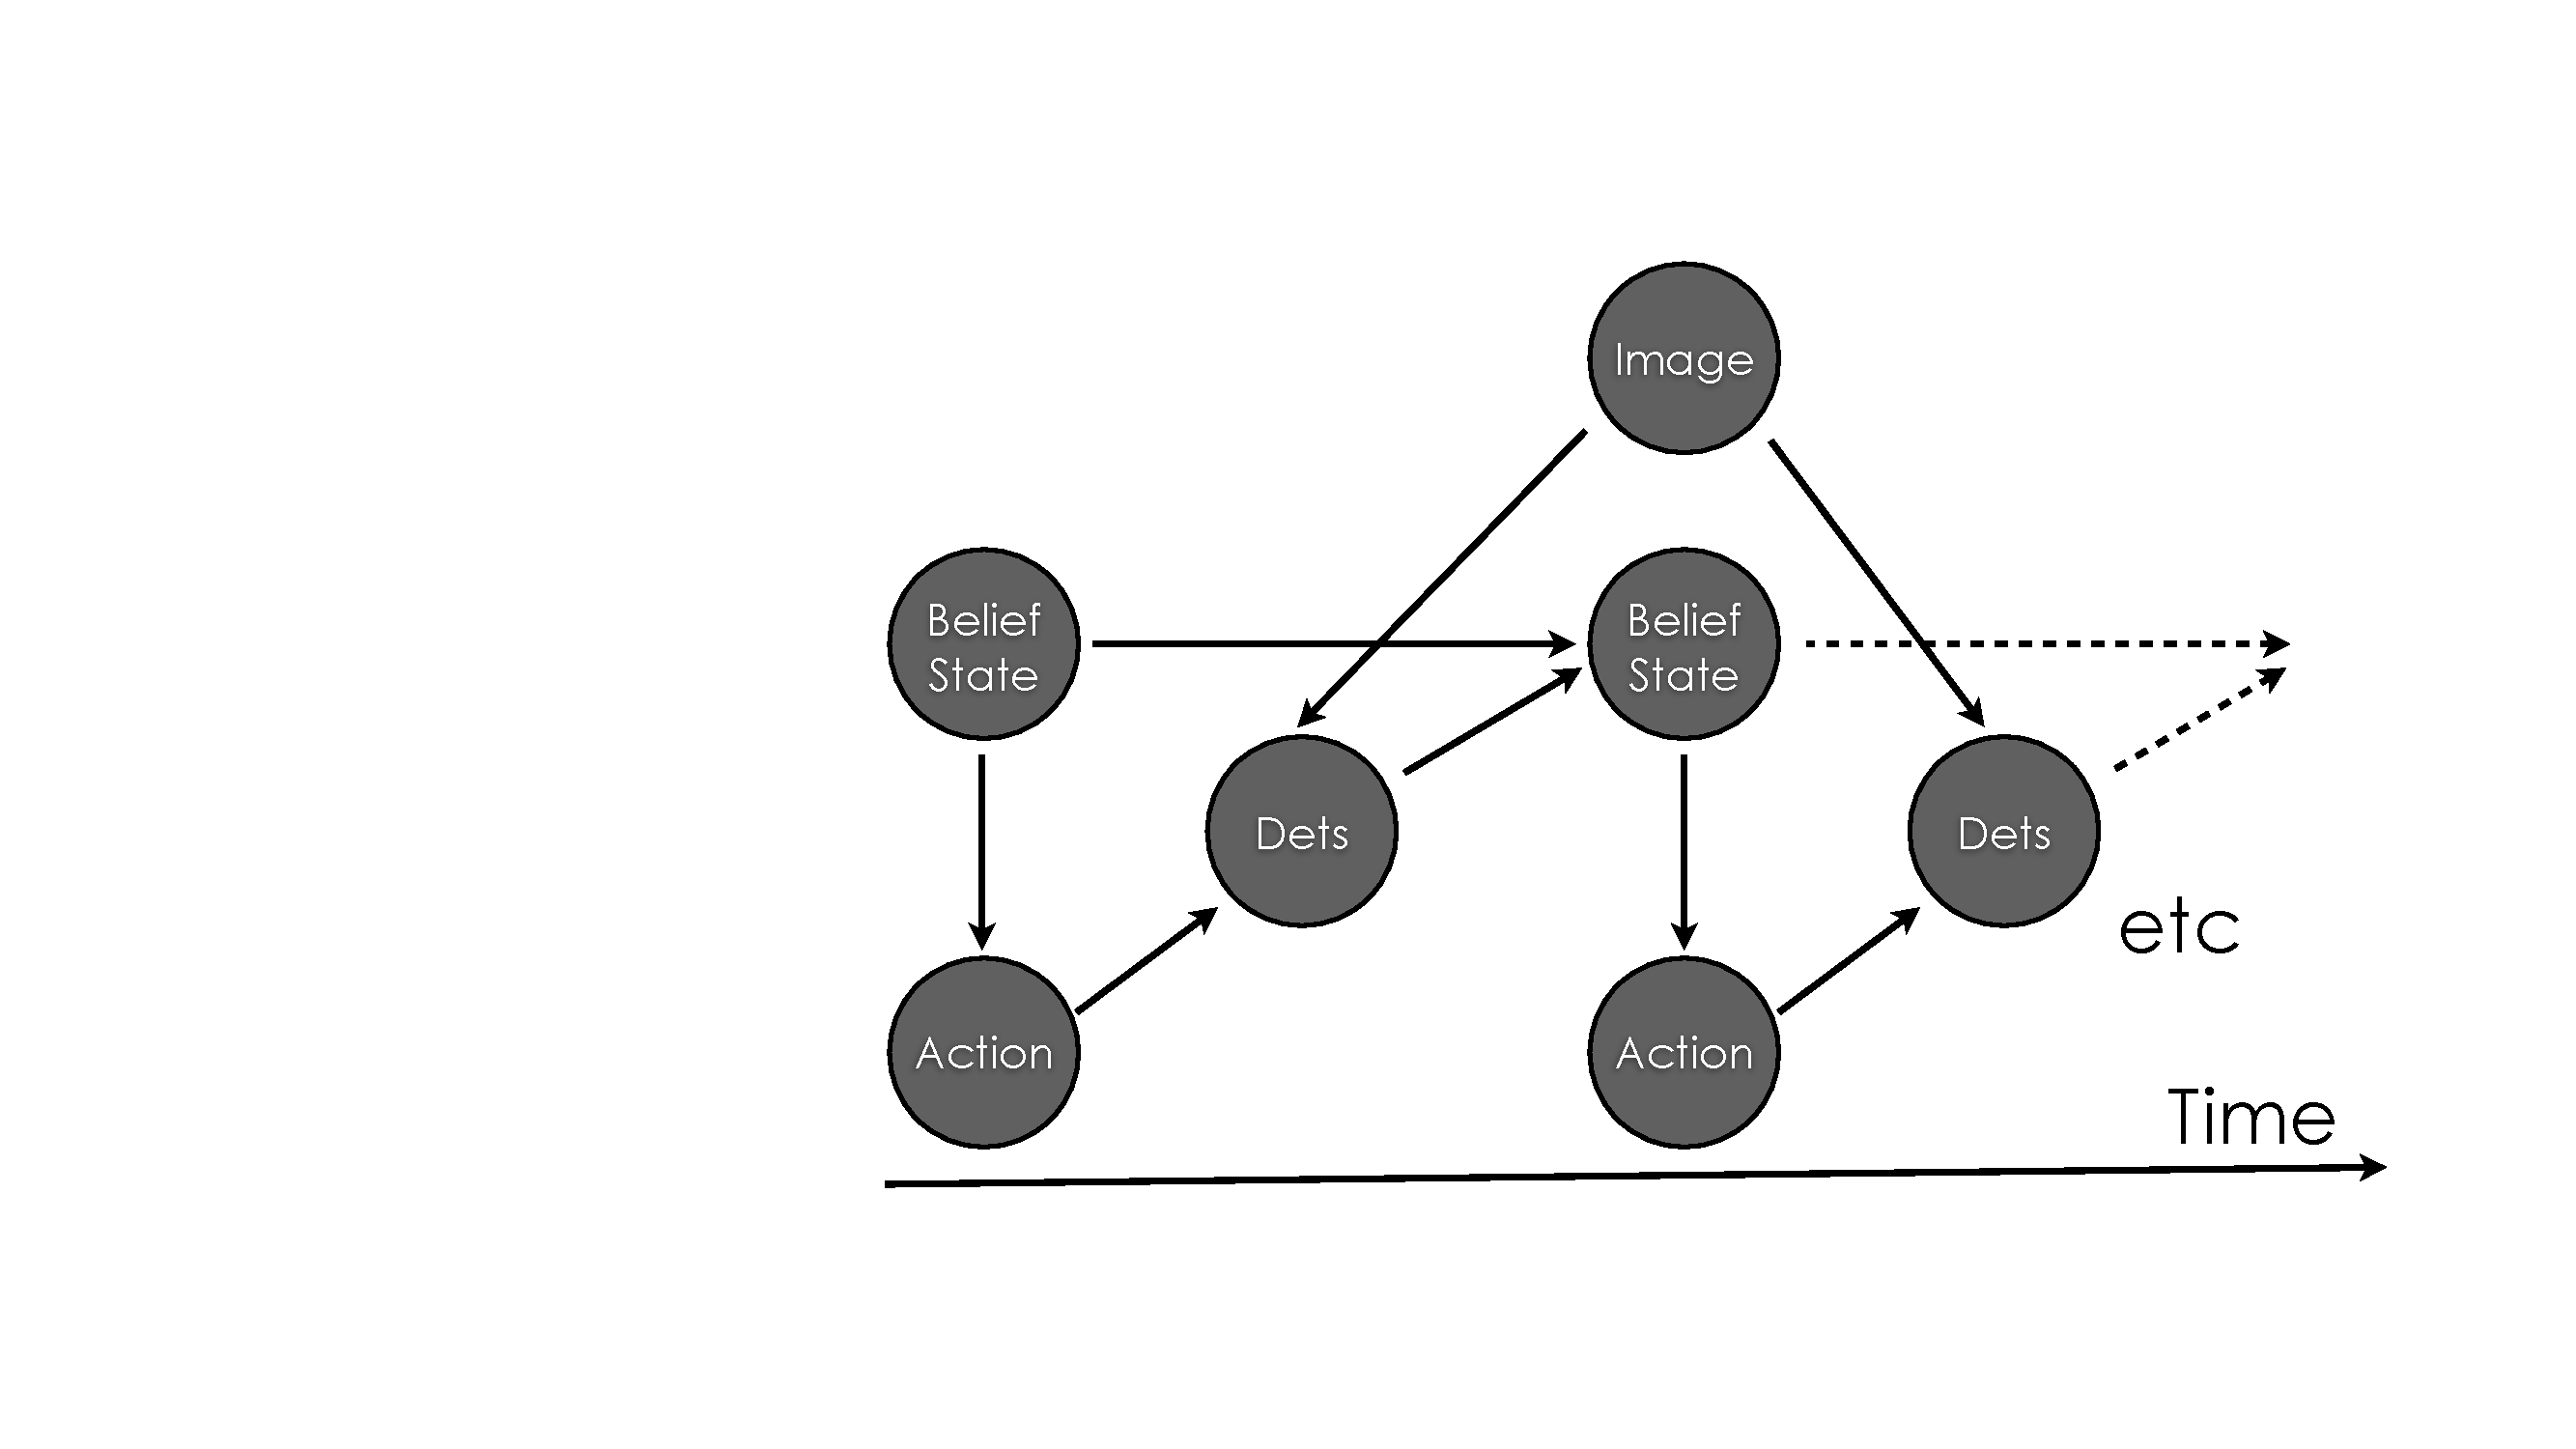
\includegraphics[width=0.9\linewidth]{../figures/pomdp.pdf}
  \caption{Summary of our approach to the problem. Our model consists of two modular parts: predicting the value of taking an action, and updating the latent belief representation having taken an action.}
  \label{fig:pomdp}
\end{figure}

Furthermore, for now we assume that $|A|=K$, the number of target classes in the dataset, so that there is exactly one detector that we can run per class.
The operation of the system, as shown in Figure~\ref{fig:pomdp}, consists in
\begin{enumerate}
\item Selecting which action to take, based on the current estimate of the image contents;
\item Updating the estimate based on the observed detections upon taking the action.
\end{enumerate}

Additionally, after every detection-generating action, the performance of the system is re-evaluated by computing the multi-class Average Precision of the updated list of detections.
This result is not observable by the policy.

We first cover the second modular part of the system: updating the latent belief representation, having already taken an action and received a list of detections.

\subsection{Belief state model}
In the terminology of partially observable decision processes, we call the part of our system that tracks progress the \emph{belief state}.
The belief state maintains inferred probabilities of object presence in the image for all classes; record of the actions taken and the composite list of resulting detections; and the current time into the episode.

In order to exploit the signal due to interobject context, we would like the object presence model to be able to model co-occurrences between object classes.
That is, if through detecting for the class 'person' we become reasonably certain that there indeed is a person in the image, this should boost the expected value of detecting for classes that tend to co-occur with 'person' in the dataset, such as 'motorcycle' or 'horse.'

The co-occurence relations between presences of all the object classes form a highly connected graph of binary random variables $C_i$, $1 \leq i \leq K$.
$C_i = 1$ if there is at least one object of class $K_i$ in the image; otherwise it is $0$.
To infer the value of each binary random variable, we use the list of detections output by a given detector.
In this paper we implement a fast, two-stage approximation to inference in this model.

We use the empirical counts of our training set to formulate initial priors of class presence, such that $P(C_i=1)$, which we write as just $P(C_i)$ for brevity, refers to the number of times class $K_i$ occurs in an image divided by the total number of images in the dataset, and $P(C_i, C_j)$ refers to the similarly normalized number of times classes $K_i$ and $K_j$ occur together in the same image.

Let's say we have inferred values $c_J$ of random variables $C_J$ where $J$ is a set of class indices.
\[
%P(C_i|C_J=c_J)=\frac
%{\sum_{c_K, K \backslash J} P(C_i, C_J=c_J | C_K=c_k)}
%{\sum_{c_K, K \backslash J} P(C_J=c_J | C_K=c_k)}
P(C_i|C_J=c_J)=\frac
{P(C_i, C_J=c_J)}
{P(C_J=c_J)}
\]

If during test time we observe a new setting of objects presences, as is likely to happen quite frequently, using empirical counts will report a probability of $0$.
Accordingly, we need to incorporate some method of smoothing the distribution over all possible assignments.

Our choice is to ``back off'' to a conditional with fewer assignments.
The complete way to do this would be to incorporate all $2^{K-1}$ conditionals of $C_i$  given any subset of the $K-1$ observed variables.
A faster approximation of the conditional is to write it out as follows:
\begin{align*}
P_{back}(C_1 | C_2\ldots C_k) = \frac{P(C_1 , C_2\ldots C_k) }{P(C_2\ldots C_k)} \\
+ \frac{\lambda_1}{K-1} \left(\sum_{i=2}^K P(C_1|C_i) \right) + \lambda_2 P(C_1)
\end{align*}

This model has three terms: the first does not assume any independeces, and relies fully on data; the second assumes the naive Bayes independence of $C_1$ and $C_i$ given any $C_j$, $i\neq j$; the third assumes that there are no dependencies between any $C_i$.
We refer to this model as \textbf{backoff}.

The model \textit{fixed policy} ignores any conditionals and just chooses the next action according to the priors of the single class:
\begin{equation*}
P_{fix}(P_1|P_2\ldots P_k) = P(C_1)
\end{equation*}

Both object class presence probability models are evaluated in Section \ref{sec:actual-evaluation}.

With a set of actions $\mathcal{A}$, progress through the belief states works as follows, starting with belief state $\mathcal{B}_0 = \emptyset$:
\begin{enumerate}
 \item Choose an action $\alpha_i \in \mathcal{A}_i$ that maximizes the value function given $\mathcal{B}_0$.
 \item Execute $\alpha_i$, receiving detections $\beta_i$. 
 \item Update the current assignments to $C_i$ with the new detections $\beta_i$.
 Update $\mathcal{B}_{i+1}$ with the new $C_i$ and the time spent on the action;
 $\mathcal{A}_{i+1} = \mathcal{A}_i\backslash \alpha_i$
 \item Repeat while $\mathcal{A}_{i+1}\neq \emptyset$ and there is time left.
\end{enumerate}
We now provide further explanation of step 3.

\subsection{Inferring $C_i$ from detections}
After executing an action, we get a set of detections: a list of bounding boxes and associated confidence scores for the given class.
We want to infer the presence of at least one object of the class in the image.
Instead of simply tresholding the scores of these detection, we extract a feature vector and classify it with an SVM.
The feature vector consists of a histogram of the values of scores and the count of detections; the parameters of the histogram are selected through cross-validation.
The featurization instead of thresholding helps in cases with no overwhelmingly confident detection, but a large number of detections nevertheless.

Table~\ref{tab:scoreClassifier} shows the performance of our classifiers for the classes of the PASCAL VOC 2007 and the two detectors used in our multiple detector system explained in Section \ref{sec:multidetector}.
We use the metric of accuracy: the number of correct decisions versus the total number of decisions.
\textit{detector} shows the results of the histogrammed CSC-classifier and \textit{detector-fast} is CSC with parameters settings to speed it up to about half the time.

\begin{table}
  \begin{center}
    \begin{tabular}{ c| c c c}
      Class & Detector & Detector-fast\\
      \hline
      aeroplane & 0.7427 & 0.5669\\
      bicycle &  0.8249 & 0.7342\\
      bird & 0.5747 & 0.5565\\
      boat &  0.6935 & 0.6565\\
      bottle  & 0.7027 & 0.6276\\
      bus &  0.5 & 0.7533\\
      car &  0.8565 & 0.7448\\
      cat & 0.6678 & 0.6213\\
      chair  & 0.7029 & 0.5\\
      cow &  0.7160 & 0.6928\\
      diningtable  & 0.6639 & 0.6393\\
      dog  & 0.5520 & 0.5281\\
      horse  & 0.8492 & 0.7077\\
      motorbike  & 0.7588 & 0.7117\\
      person &  0.8063 & 0.7263\\
      %\vdots&\vdots&\vdots&\vdots \\
      pottedplant  & 0.6213 & 0.6115\\ 
      sheep &  0.6978 & 0.6336\\ 
      sofa &  0.6803 & 0.5901\\ 
      train  &  0.8163 & 0.7149\\ 
      tvmonitor & 0.7622 & 0.7066
    \end{tabular}
    \caption{Per-class accuracies of the object presence classifier. Input is a set of detections on an image, output by either the baseline or the \emph{fast} detector.}
    \label{tab:scoreClassifier}
  \end{center}
\end{table}




\subsection{Value Function and the Definition of Rewards}
Having updated the belief state, the system must again pick the next action.
Remember that our system aims to maximize the single-number metric of the area under the AP vs. Time curve.
Accordingly, we define the final reward accrued by a policy to be precisely the area under the curve between start and deadline times.

\begin{figure}[htb]
  \center{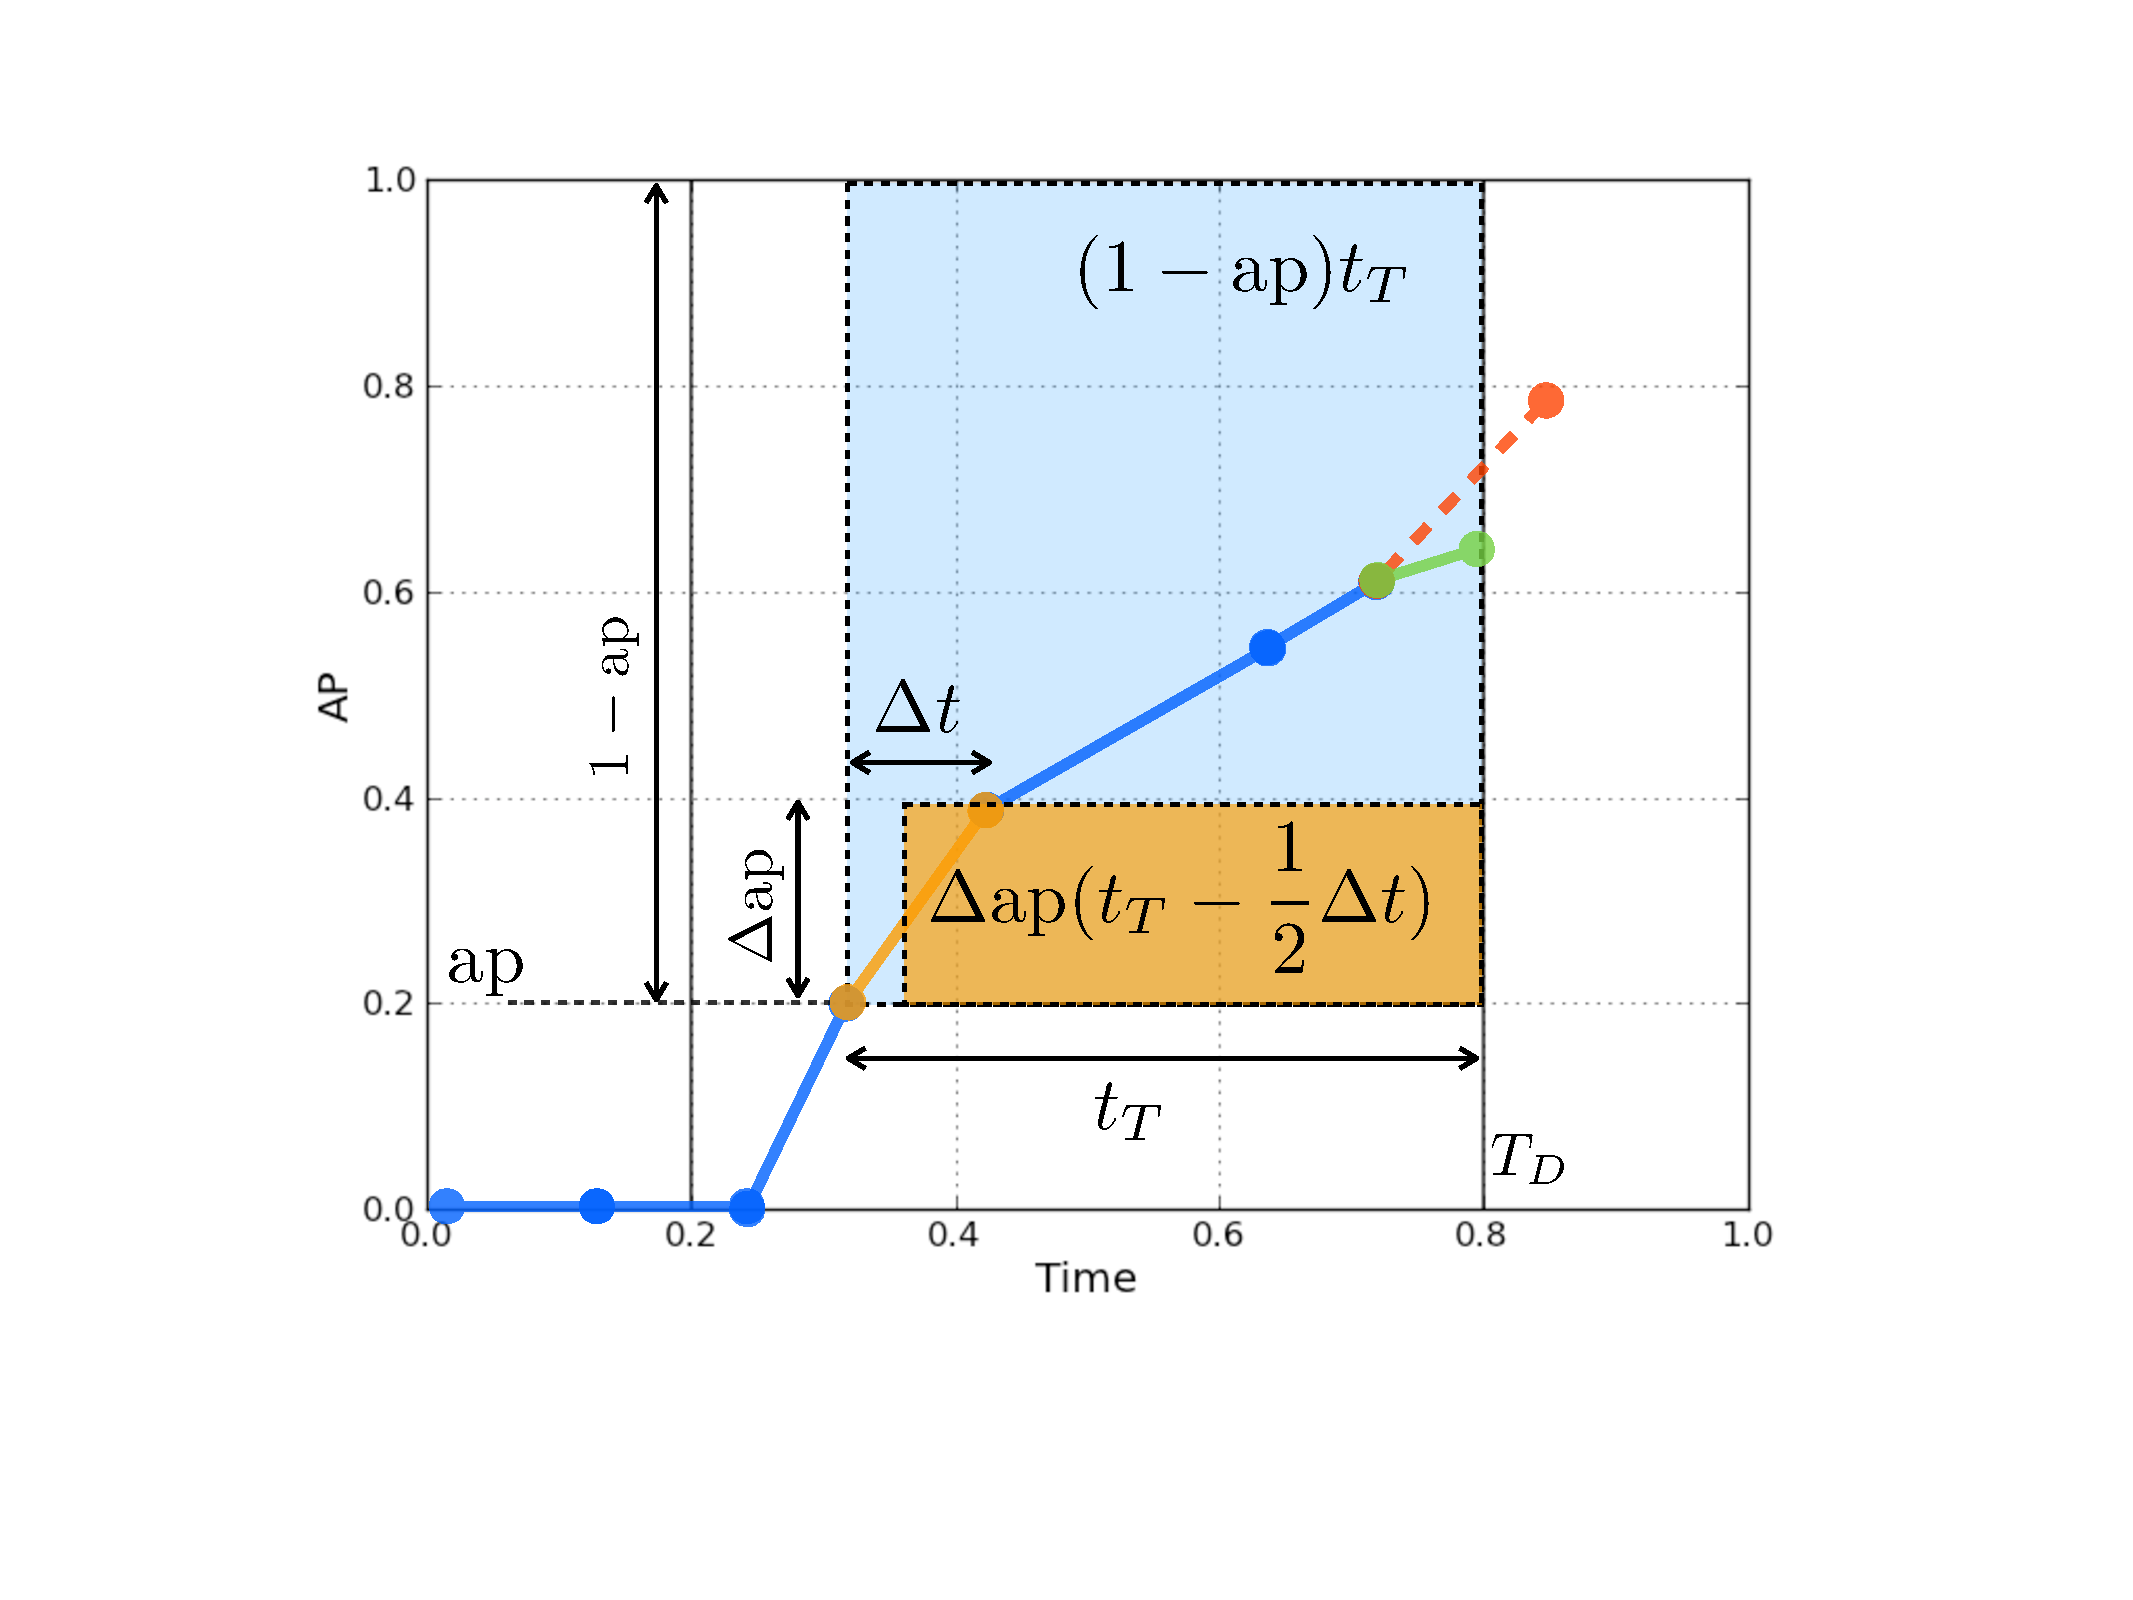
\includegraphics[width=1\linewidth]{figures/apvst_expl.pdf}}
  \caption{\label{fig:rewards}A per-action greedy value function that corresponds to the maximization of our objective function is the ratio of the area of the horizontal slice under the curve due to the action to the maximum possible area the action could have captured. The figure shows this analysis for the action highlighted in orange.}
\end{figure}

The final reward of the policy should be the summation of individual rewards accrued by each action.
Our choice, shown in Figure~\ref{fig:rewards}, is the area of a horizontal ``slice'' of the area under the curve due to the action.

Specifically, we define the reward of an action as
\begin{equation}\label{eq:advanced}
\Delta AP (t_T-\Delta t)
\end{equation}
where $t_T$ is the time left until deadline, and $\Delta t$ and $\Delta AP$ are the time taken and AP change produced by the action.

The equation breaks down into a term to maximize, $\Delta AP t_T$, and a term to minimize, $\Delta AP \Delta t$.
This agrees with the intuition that to capture the most area under the curve, the slope needs to be maximized at each point.
Additionally, the equation shows that if $\Delta t$ exceeds $t_T$, the value of taking the action is negative.
This is good, as these actions don't actually contribute detections to the final evaluation.

We can accentuate the desire for high slope in a value function with the same properties:
\begin{equation}\label{eq:slope}
\frac{\Delta AP}{\Delta t} (t_T - \Delta t)
\end{equation}
This function always maximizes the slope, except for when doing so would lead to taking more time than alloted by the deadline.
(Consider the branching of the performance curve in \ref{fig:rewards} into green and red branches when it approaches the deadline.
The branches represent two actions of the case where maximizing slope would not be the correct behavior.)

Of course, we cannot be aware of the true value of $\Delta t$ until having taken the action, and the policy can never be fully certain of the value of $\Delta AP$.
When estimating the value function, we therefore use the expected values of these terms.

$\Delta t_{avg}$ is the average running time of the detector on an image, estimated on a validation set of the data at training time.
$\Delta AP$ is estimated as $\Delta AP_{avg} P(C)$, where $P(C)$ is the current belief in the presence of class $C$ in the image, and $\Delta AP_{avg}$ is the ``naive'' AP contribution averaged over images containing class $C$.

During training time, we learn the behavior of different detectors: the average time taken per image, and the average AP contribution on images that do and do not contain any objects of the desired class.
For the latter statistic, we collect two variants.
The ``naive'' AP contribution is the performance of the detector in the multi-class regime if its detections were added to an empty set of detections.
That is, true detections cannot become false positives due to being overshadows by a more confident but wrong detection of a different class in this evaluation.

The ``actual'' AP contribution is the real performance of the detector in the multi-class regime: its detections are added to an existing set of detections, unless it was the result of the first action to run.
This case, although more realistic, is subject to signficant noise due to other detectors' performance that may obscure the evaluated detector's characteristics.


We additionally experimented with estimating $\Delta AP$ as $\Delta AP_{avg|present} P(C) + \Delta AP_{avg|absent} (1-P(C))$, but the results were worse than with the given equation.


\section{Evaluation of the System} \label{sec:actual-evaluation}
Our system treats the detector as a black box that takes an image and class and returns a list of detections for that class.
In our implementation, we use the Cascaded Deformable Part Model detector, which is among both the fastest and most robust detectors currently available \cite{Felzenszwalb2010a}.
The detectors take on average around one second to process a standard dataset image.

We evaluate on the standard PASCAL VOC 2007 detection task dataset \cite{pascal-voc-2010}.
We note that the dataset is not known for having high levels of signal in the inter-object and scene-object context \cite{Divvala2009}, so the parts of our model that seek to exploit inter-object context may be at a disadvantage.
We follow the approach set forth in Section \ref{sec:evaluation}, but set the start time at $0$ and ignore the feature computation time.

During training time, we learn the behavior of different detectors: the average time taken per image, and the average AP contribution on images that do and do not contain any objects of the desired class.
For the latter statistic, we collect two variants.
The ``naive'' AP contribution is the performance of the detector in the multi-class regime if its detections were added to an empty set of detections.
That is, true detections cannot become false positives due to being overshadows by a more confident but wrong detection of a different class in this evaluation.

The ``actual'' AP contribution is the real performance of the detector in the multi-class regime: its detections are added to an existing set of detections, unless it was the result of the first action to run.
This case, although more realistic, is subject to signficant noise due to other detectors' performance that may obscure the evaluated detector's characteristics.

In Figure \ref{fig:1det}, the ``Oracle'' curve is obtained by running detectors in the order of greatest ``naive'' AP contributions on each image.
The performance is formidable, which suggests that the ``naive'' statistics is worth using in our policies.

Due to the large disparity in performance between detectors for different classes, it is not surprising that the curve of the ``Oracle'' policy turns downward: after obtaining the initial true positives, the policy has no choice but start running worse-performing detectors which generate false positives, bringing the overall AP down.

\begin{figure*}[htb]
  \center{\includegraphics[width=\textwidth]
      {figures/det1.pdf}}
  \caption{\label{fig:1det} The random policy shows the typical path of an uninformed multi-class detector through the image, while the oracle policy shows the room to improve. Our policy results in performance between the two, showing clear improvement over the random baseline.}
\end{figure*}

\section{Policy with multiple detectors per class} \label{sec:multidetector}
We now expand our model to deal with being able to run multiple detectors per class.
We simulate a faster but less robust detector, as would be obtained by modifying the stride or classifier strength, by randomly taking half of the detections output by our base detector, described below in Section \ref{sec:actual-evaluation}.

Simply adding such a detector to the existing system as described would lead to pathological performance.
For example, let's assume that the image contains an object of class 'dog;' we run our most powerful detector for that class and thereafter update our belief state with the strong posterior of this class presence.
Our value function estimates for running the other 'dog' detectors are now increased from before, despite the fact that actually running them is unlikely to produce any new true positives and will in fact probably hurt performance due to false positives.
(Remember that in our evaluation, a ground truth object may only be matched to one detection proposal---all other detections matching that ground truth are considered false positives.)

For this reason, we augment the value function with this consideration.
The only change that needs to be made is to the expected score increase:
\begin{equation}\label{eq:multiclass}
\mathbb{E}[\Delta AP^i] = P(C)\Delta AP^i_{avg} - P(C)\sum_{j \neq i} \delta_j \Delta AP^j_{avg}
\end{equation}
where $\Delta AP^i$ is the score increase of the detector belonging to the action under consideration, the sum is over all other detector actions of the same class as $i$, and $\delta_j$ is an indicator function for whether action $j$ has been taken.

\begin{figure*}[htb]
   \center{\includegraphics[width=\linewidth]
       {figures/det2.pdf}}
  \caption{\label{fig:2det} When using multiple detectors per class, there is a clear benefit to using a policy that is sensitive to the finite amount of reward that can be obtained from a single class.}
\end{figure*}

Figure \ref{fig:2det} shows the performance comparison of the usual random, oracle, and the two evaluated policies.

Although we do not evaluate this, our system allows for setting priority weights on different detector classes; this results in different policy behaviors.
